



\chapter{Inelastic Collisions in MD}


As we already saw in \ref{sec:collapse}, incelasticity is often not just a small unnecessary correction to a well-behaved and converging mathematical method. Many systems do not converge, if \textbf{dissipation} is not taken into account. From landslides to turbulent flow in aircraft engines, energy loss and dissipation are very often necessary for the simulations to be stable and useful for the practice. This is why in this chapter we will briefly go back to the MD methods we discussed before defining event driven programming and the two concepts will be slightly modified and adapted to solve this issue. After having treated simple models like \textbf{damped oscillators} and \textbf{plastic deformation}, \textbf{inelasticity} in the context of the \textbf{inelastic collapse} is treated on a very basic conceptual level. 

As a new approach to a particular class of situations, \textbf{Contact dynamics}, is introduced. As a brief repetition of concepts treated in ICP \citep{comp_phys} with some brief discussion of new methods, \textbf{particles in fluids} concludes the chapter.

\section{Damped Oscillator}
Inelasticity can be easily introduced in MD simulations that are not based on event driven algorithms. For this we will make use of a one dimensional damped oscillator. The equation of motion of the damped oscillator should be known from classical mechanics. Using the radial distance between two particles $r\equiv R_i +R_j -\abs{\vec{x}_i-\vec{x}_j}$ and the effective mass $m_{\text{eff}} = \frac{m_1m_2}{m_1 + m_2}$, the force between them is given by

\begin{equation}
 f = -kr -\gamma \dot{r}= m_{\text{eff}}\ddot{r}
\end{equation}

\vspace{0.3cm}
\noindent
the solution of which is 
\begin{equation}
r\kl{t} = \frac{v^{\text{before}}}{\omega} \sin\ekl{\omega t} \exp\ekl{-\delta t}
\end{equation}
where  $\omega = \sqrt{\omega_0^2 - \delta^2}$ is the oscillator frequency, $\omega_0 = \sqrt{\frac{k}{m_{\text{eff}}}}$ is the ground frequency of the undamped oscillator, and $\delta = \frac{\gamma}{2m_{\text{eff}}}$ is the damping factor. Whenever an oscillator is damped the frequency is shifted, thus the period is generally larger.

We can regard the collisions as a single cycle in a damped oscillator, where some energy is dissipated due to the damping. The period of the oscillator is made up by the approaching and repulsion phase. The collision (half of the approaching phase and repulsion respectively) lasts half the period of an oscillation, and when the particle bounces back it will not reach the same kinetic energy it had before the collision. We can therefore calculate the restitution coefficient if we compute the velocities before and after the impact:

\begin{equation}
 e_n = \frac{\dot{r}\kl{t+T}}{\dot{r}} = \exp\ekl{-\delta T} = \exp\ekl{- \frac{\gamma \pi}{\sqrt{  4 m_\text{eff} k - \gamma^2  }}} 
\end{equation}
Here we used that the particle takes half a period  to reach the closest point to the other particle: $T= \frac{\pi}{\omega}$ and plugged in the $\omega$ of the classical damped oscillator. From this relation we can compute the damping factor with the knowledge of the restitution coefficient:
\begin{equation}
\gamma = 2 \ln{\kl{e_n}} \sqrt{\frac{m_{\text{eff}}k}{\text{ln}^2\kl{e_n}+\pi^2}}
\end{equation}


An important assumption that has been made is that the restitution coefficient is constant throughout the complete interaction. For this reason, we can describe the dissipation with a viscous damping $\gamma$. This is not true for e.g. Hertzian Contact: when real spheres interact and their shape is altered. In every collision, some kinetic energy  is lost due to plasticity. The problem is that for spheres the amount of energy lost has a non trivial dependence on  the overlap. This implies also a dependency on the previous interactions and the collision history that already altered the spheres' shape. Thus the restitution coefficient is not constant and the aproach has to be corrected.






\section{Plastic Deformation}

Here we consider a very important case in mechanics and engineering: the irreversible change in the shape of an object after an interaction, \emph{plastic deformation} (see Fig. \ref{fig:plasticity1}). If the interaction is completely elastic then the plasticity is not important. However, in many fields, this is not very often the case. In engineering and industry, plastic deformation is a very important issue. 


\vspace{0.1cm}
\noindent
\begin{minipage}{.95\textwidth}
  \begin{minipage}{\textwidth}
    \centering
    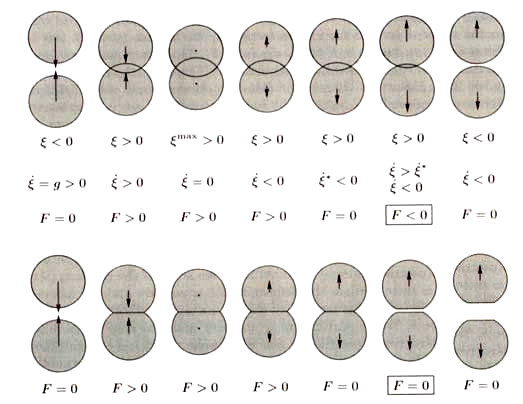
\includegraphics[width=.85\textwidth]{pics/plasticity1.jpeg}
    \captionof{figure}{Completely elastic and plastic interactions. Note that the forces differ.}
    \label{fig:plasticity1}
  \end{minipage}
\hfill
  \begin{minipage}{0.05\textwidth}
\,
  \end{minipage}
\end{minipage}
\vspace{0.1cm}




The easiest approach to model plasticity is the one introduced by Walton and Braun \citep{walton}. They approximate the collision event as two separate interactions between springs, where the stiffness is different for the repulsion. This results in hysteretic and nonlinear behaviour. In particular, the interaction is dissipative and non elastic. Fig. \ref{fig:plasticity2} schematically depicts the process: first the objects approach following Hook's law and overlap up to $\delta_\text{max}$. During this time the objects are deformed and therefore repulsion occurs with a different spring constant such that the repulsive forces are gone before the overlap parameter has vanished.

 



\vspace{0.1cm}
\noindent
\begin{minipage}{\textwidth}
\begin{minipage}{\textwidth}
  \centering
  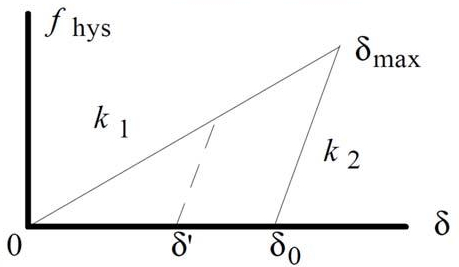
\includegraphics[width=.55\textwidth]{pics/deformation.jpeg}
  \captionof{figure}{Elastic approximation of an inelastic collision after \citet{walton}.}
  \label{fig:plasticity2}
\end{minipage}
\end{minipage}
\vspace{0.1cm}


Mind that the collision time is not symmetric, since loading lasts longer than unloading:
\begin{equation}
t_c = \frac{\pi}{2} \kl{ \sqrt{\frac{m_{i,j}}{k_1}} + \sqrt{\frac{m_{i,j}}{k_2}}  }.
\end{equation}
The dissipated energy can be calculated by integrating the area enclosed by the two curves. From this we obtain the restitution coefficient
\begin{equation}
r= \frac{E^{\text{after}}}{E^{\text{before}}} = \frac{k_1}{k_2}
\end{equation}




\section{Coulomb Friction and Discrete Element Method}


Another source of dissipation is friction. The energy loss in Coulomb friction is proportional to the normal force. The classic example of Coulomb friction is the slide on an inclined chute. As probably known from beginner's lectures there are to friction coefficients, the static and the dynamic coefficient. The first is valid if the object is not moving, it represents the force that one needs to bring the object into movement. The second coefficient represents the friction once the object is already moving. At a certain inclination angle, the \emph{friction angle}, the object will begin to slide down the chute. The tangent of the angle gives the static friction coefficient. An important fact, is that all the motion is independent on the contact area. Numerically the problem is very unpleasent since the friction coefficient $\mu$   is described by a function which is not continuous: for $v\ne 0$ the value is a constant ($\mu=\mu_d$), and for $v=0$ it assumes another value ($\mu= \mu_s$).



The first approach \citep{luding} is to distinguish between a small shear velocity below which one can implement static friction and above which one has to implement dynamic friction:

\begin{align*}
\Delta p_t &= m_{\text{eff}} \kl{e_t+1}\underbrace{\kl{\vec{v}_i^{\,\text{before}}-\vec{v}_j^{\,\text{before}}}}_{v_t}\vec{t} \hspace{0.5cm} \text{for }v_t << 1 \\
\Delta p_t &= \mu_d m_{\text{eff}} \kl{e_t+1}\kl{\vec{v}_i^{\,\text{before}}-\vec{v}_j^{\,\text{before}}}\vec{n} \hspace{0.5cm} \text{for }v_t >> 1 \\
\end{align*}


If one has a set of particles interacting via friction (e.g. sand or stones), the method proposed by Cundall  \citep{cundall} is nowadays a standard. This forward integration technique is widely used for engineering and in industry (e.g., the company founded by Cundall itself, \emph{Itasca}, is the leading provider of software that works on this method).


Similarly to the method mentioned before we introduce two terms for the strength, one for the static and one for the dynamic interaction. 

\begin{align}
f_t &= - \text{min}\ekl{\gamma v_t, \mu_d f_n} \text{sign} \ekl{v_t} \\
f_t &= - \text{min}\ekl{\abs{k_s\xi}, \mu_s f_n} \text{sign} \ekl{v_t}
\end{align}

The difference from the method used before is the behaviour of the particles if their velocities are very small. If the velocities are smaller than a certain value, then a spring is applied by introducing an elastic force with constant $k_s$. If $\abs{k_s\xi}> \mu_sf_n$, then the spring is removed and the particles are free to move with the static or dynamic friction coefficient depending on their velocity.  






